\chapter{Конструкторская часть}
В этом разделе будут приведены схемы алгоритмов и вычисления трудоемкости
исследуемых алгоритмов сортировки.

\section{Разработка алгоритмов}

На рисунках  \ref{fig:bts}, \ref{fig:radix} и \ref{fig:beads}
представлены схемы алгоритмов сортировки бирнарным деревом, поразрядной и бусинами
соответственно.

\begin{figure}[h!]
    \centering
    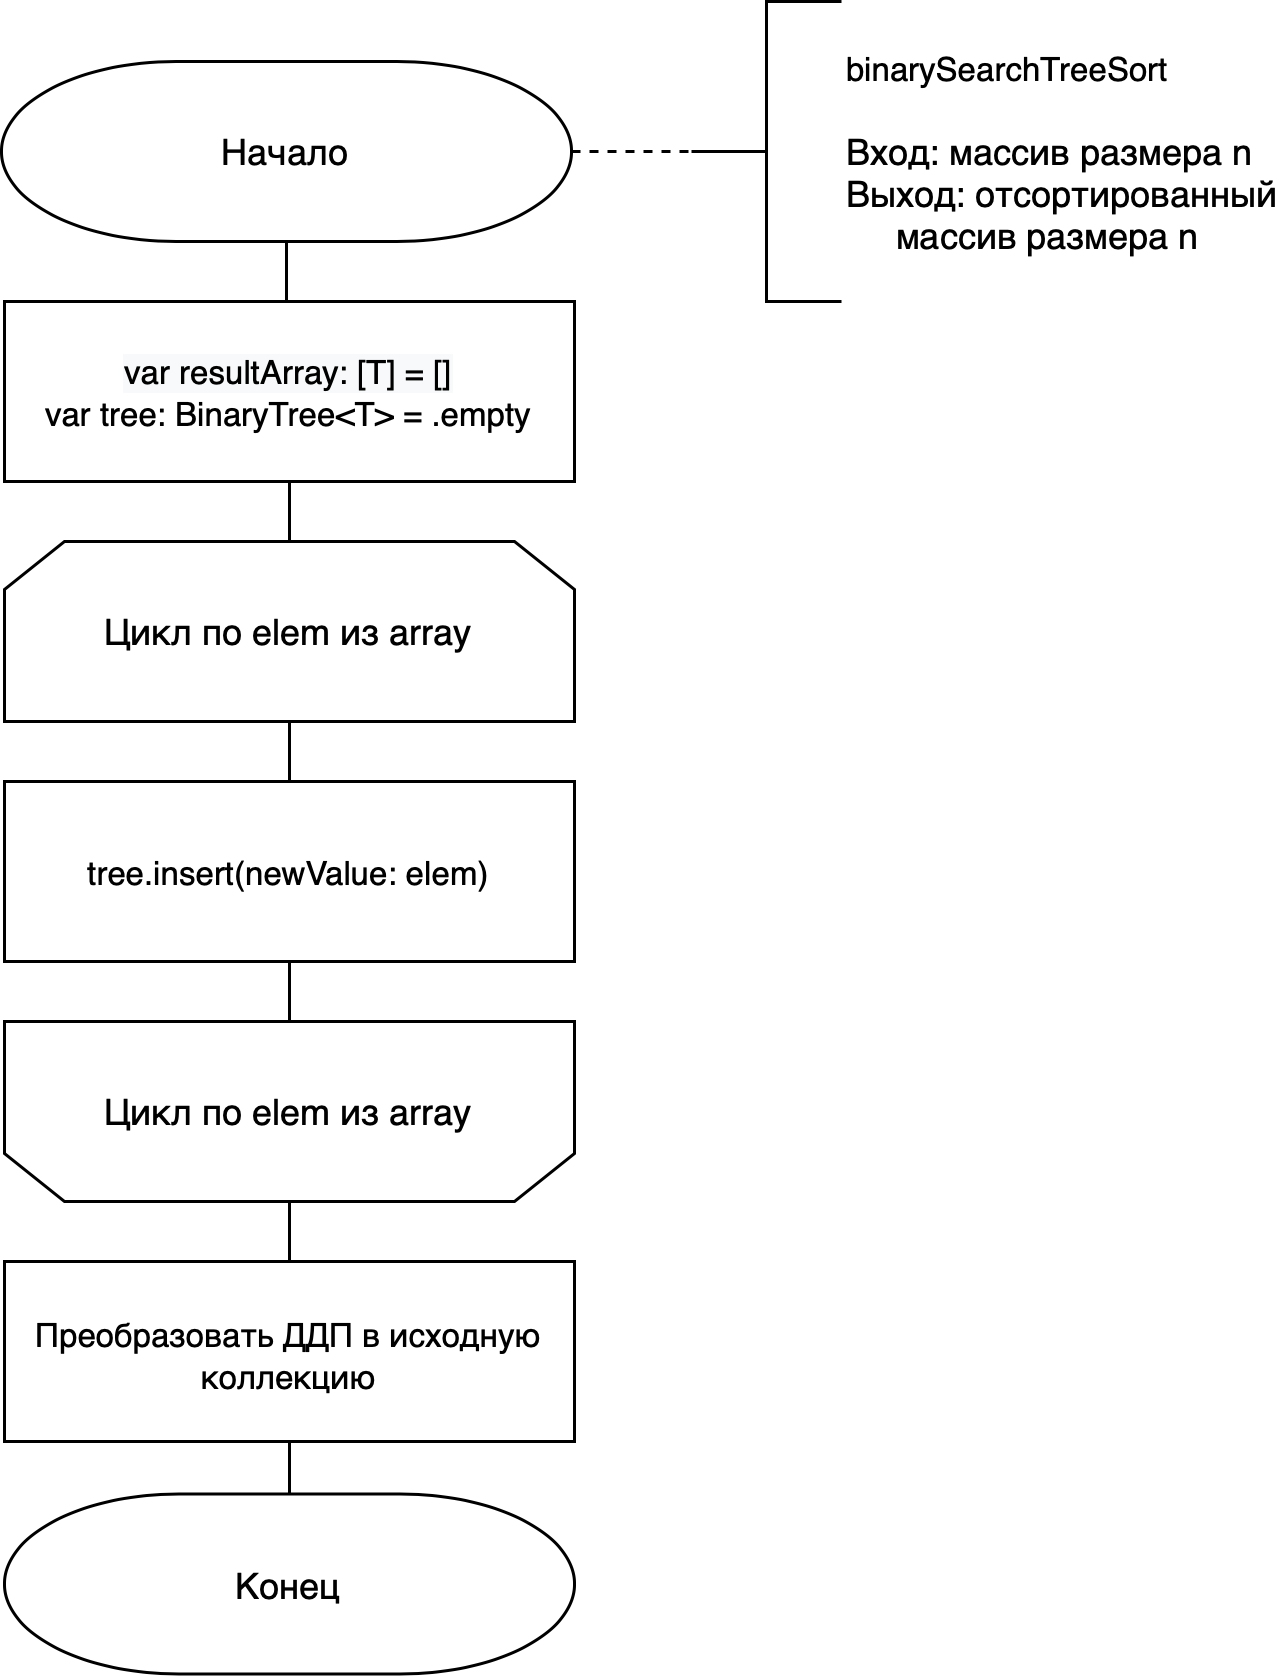
\includegraphics[width=0.7\linewidth]{inc/img/bt_sort}
    \caption{Схема алгоритма сортировки бинарным деревом}
    \label{fig:bts}
\end{figure}

\begin{figure}[h!]
    \centering
    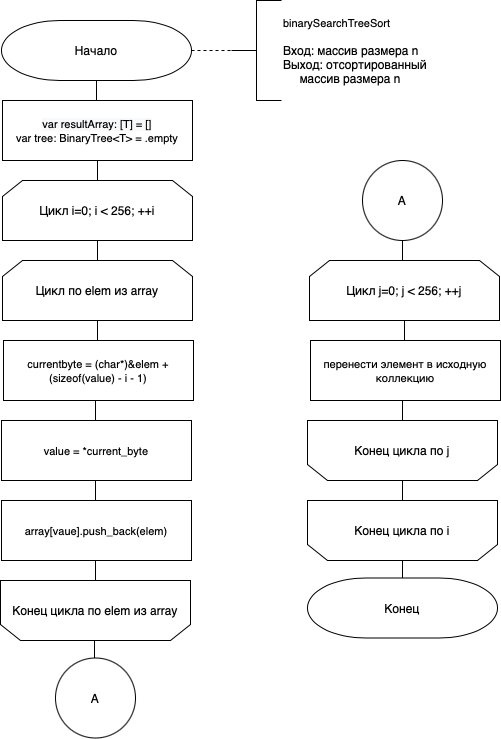
\includegraphics[width=0.8\linewidth]{inc/img/radix_sort}
    \caption{Схема алгоритма побитовой сортировки}
    \label{fig:beads}
\end{figure}

\begin{figure}[h!]
	\centering
	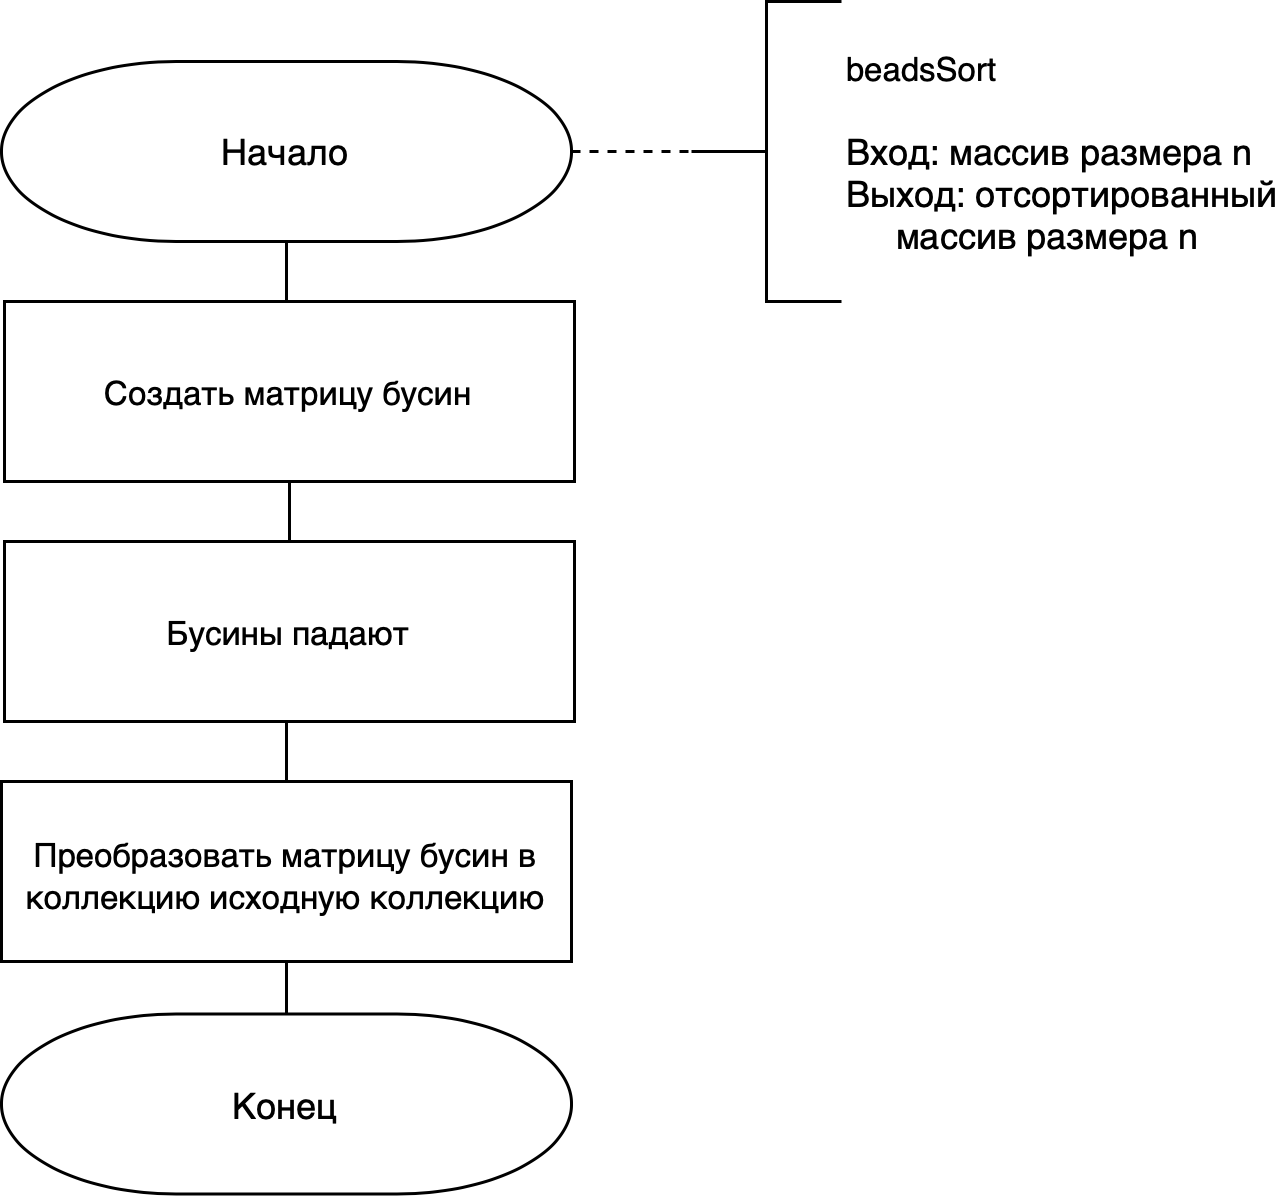
\includegraphics[width=0.8\linewidth]{inc/img/bead_sort_3}
	\caption{Схема алгоритма сортировки бусинами}
	\label{fig:radix}
\end{figure}
\clearpage

\section{Установка модели вычислений для оценки трудоемкости}

Для оценки трудоемкости введем следующую модель вычислений:
\begin{enumerate}
    \item операции из списков (\ref{for:operators_1},~\ref{for:operators_2}) имеют трудоемкость 1;
    \begin{equation}
        \label{for:operators_1}
        +, -, /, *, \%, =, +=, -=, *=, /=, \%=
    \end{equation}
    \begin{equation}
        \label{for:operators_2}
        ==, !=, <, >, <=, >=, [], ++, {-}-, ->, !
    \end{equation}
    \item трудоемкость оператора выбора \code{if условие then A else B} рассчитывается, как (\ref{for:if});
    \begin{equation}
        \label{for:if}
        f_{if} = f_{\text{условия}} +
        \begin{cases}
            f_A, & \text{если условие выполняется,}\\
            f_B, & \text{иначе.}
        \end{cases}
    \end{equation}
    \item трудоемкость цикла рассчитывается, как (\ref{for:for});
    \begin{equation}
        \label{for:for}
        f_{for} = f_{\text{инициализации}} + f_{\text{сравнения}} + N(f_{\text{тела}} + f_{\text{инкремент}} + f_{\text{сравнения}})
    \end{equation}
    \item трудоемкость вызова функции равна 0;
    \item трудоемкость выделения памяти на куче равна 10.
\end{enumerate}

\section{Трудоёмкости алгоритмов}

Обозначим $N$ - количество элементов в коллекции, которая поступает на вход.

\subsection{Алгоритм сортировки бинарным деревом}

Будем называть дерево сбалансированным, если для каждого поддерева
высота его поддеревьем различается не более чем на 1.


Аналогично будем называть дерево абсолютно несбалансированным, если у каждого
поддерева есть лишь один потомок.

\begin{itemize}
    \item Прверка на пустой массив имеет трудоемкость:
    \begin{equation}
        \label{for::binary_tree_empty}
        f_{empty} = 1
    \end{equation}
    \item Трудоемкость цикла вставки в бинарное дерево:
    \begin{equation}
        \label{for::binary_tree_insert_cycle}
        f_{cycle} = 1 + 2N + N \cdot f_{insert}
    \end{equation}
    \item Трудоемкость операции вставки $i$-го элемента в сбалансированное бинарное дерево (лучший случай):
    \begin{equation}
        \label{for::binary_tree_insert_best_case}
        f_{insert best} = 9(\lfloor{log_2 i}\rfloor - 1) + 28
    \end{equation}
    \item Трудоемкость операции вставки $i$-го элемента в абсолютно несбалансрованное бинарное дерево (худший случай):
    \begin{equation}
        \label{for::binary_tree_insert_worst_case}
        f_{insert worst} = 9i + 28
    \end{equation}
    \item Трудоемкость преобразования бинарного дерева в коллекцию:
    \begin{equation}
        \label{for::binary_tree_to_container}
        f_{cont} = N \cdot (11 log_2 N  + 26)  + 15
    \end{equation}
\end{itemize}

Трудоемкость в лучшем случае будет равна:
\begin{equation}
    \label{for:binary_tree_best_1}
    f_{best} = 1 + 1 + 2N + N \cdot (18 log_2 N + 19) + N \cdot (11 log_2 N  + 26)  + 15 =
\end{equation}
\begin{equation}
    \label{for:binary_tree_best_2}
    = 29 N log_2 N + 47N 17 = O(N log N)
\end{equation}

Трудоемкость в худшем случае будет равна:
\begin{equation}
    \label{for:binary_tree_worst_1}\
    f_{worst} = 1 + 1 + N + N \cdot \frac{28 + (8N + 28)}{2} + N \cdot (11 log_2 N  + 26)  + 15 =
\end{equation}
\begin{equation}
    \label{for:binary_tree_worst_2}
    = 4N^2 + 11 N log_2 N + 55N + 17 = O(N^2)
\end{equation}


\subsection{Алгоритм сортировки бусинами}


Стоит отметить, что рассматривается сортировка бусинами, для
неотрицательных чисел. Введем $S$ - значение наибольшего элемента
сортируемой коллекции.


\begin{itemize}
    \item Трудоёмкости вычисления размера контейнера:
    \begin{equation}
        \label{for:bedads_container_size}
        f_{size} = 4N
    \end{equation}
    \item Тредоемкость нахождения максимального значения:
    \begin{equation}
        \label{for:selection_inner}
        f_{max value} = 3N
    \end{equation}
    \item Трудоемкость построения матрицы:
    \begin{equation}
        \label{for:selection_if}
        f_{matrix} = 2 + 8N + 4SN
    \end{equation}
    \item Трудоемкость осуществления падения бусин в лучшем случае:
    \begin{equation}
        \label{for:fallbest}
        f_{fallbest} = 2 + 8N + 3SN
    \end{equation}
    \item Трудоемкость осуществления падения бусин в худшем случае:
    \begin{equation}
        \label{for:fallworst}
        f_{fallworst} = 2 + 8N + 4SN
    \end{equation}
    \item Трудоемкость перевода бусин к исходной коллекции в лучшем случае:
    \begin{equation}
        \label{for:tocontainerbest}
        f_{tocantainerbest} = 2 + 5N + 3SN
    \end{equation}
    \item Трудоемкость перевода бусин к исходной коллекции в худшем случае:
    \begin{equation}
        \label{for:tocontainerworst}
        f_{tocantainerworst} = 2 + 5N + 4SN
    \end{equation}
\end{itemize}

Трудоемкость в лучшем случае будет равна:
\begin{equation}
    \label{for:beads_1}
    f_{best} = 5 + 19N + 15SN = O(S \cdot N)
\end{equation}

Трудоемкость в худшем случае будет равна:
\begin{equation}
    \label{for:beads_2}
    f_{worst} = 5 + 19N + 13SN = O(S \cdot N)
\end{equation}

\subsection{Алгоритм побитовой сортировки}


Стоит отметить, что рассматривается побитовая сортировка, для
неотрицательных целых чисел. Введем $w$ - количество байтов,
которое занимает наимбольшей элемент сортируемой коллекции.


Трудоемкость в лучшем и худшем случае будет равна:
\begin{equation}
    \label{for:beads_1}
    f = 1294 wN + 1285wN + 2 = O(w \cdot N)
\end{equation}

\section*{Вывод}

Разработаны схемы 3 алгоритмов сортировки. Получена теоритическая оценка
трудоемкости каждого алгоритма.
